\documentclass[pdflatex,sn-mathphys-num,referee,lineno]{sn-jnl}

\newcommand{\proglang}[1]{\textit{#1}}
\newcommand{\code}[1]{\texttt{#1}}
\newcommand{\pkg}[1]{\textbf{#1}}

\usepackage{amsmath}
\usepackage[section]{placeins}
\usepackage{amsfonts}
\usepackage{amssymb}
\usepackage{booktabs}

\begin{document}

\title[\pkg{TCA} (Trajectory Clustering Analysis): A \proglang{Python} Package for Clustering Unidimensional and Multidimensional Care Trajectories]{%
  \pkg{TCA} (Trajectory Clustering Analysis): A \proglang{Python} Package
  for Clustering Unidimensional and Multidimensional Care Trajectories}

\author*[1,2]{\fnm{First} \sur{Author}}\email{iauthor@gmail.com}

\author[2,3]{\fnm{Second} \sur{Author}}\email{iiauthor@gmail.com}
\equalcont{These authors contributed equally to this work.}

\author[1,2]{\fnm{Third} \sur{Author}}\email{iiiauthor@gmail.com}
\equalcont{These authors contributed equally to this work.}

\affil*[1]{\orgdiv{Department}, \orgname{Organization}, \orgaddress{\street{Street}, \city{City}, \postcode{100190}, \state{State}, \country{Country}}}

\affil[2]{\orgdiv{Department}, \orgname{Organization}, \orgaddress{\street{Street}, \city{City}, \postcode{10587}, \state{State}, \country{Country}}}

\affil[3]{\orgdiv{Department}, \orgname{Organization}, \orgaddress{\street{Street}, \city{City}, \postcode{610101}, \state{State}, \country{Country}}}

\abstract{%
\textbf{Background:} Healthcare trajectory analysis is a key challenge in public health, but such data remain difficult to exploit due to the temporal ordering of events and their possible co-occurrence. 
Open-source tools for trajectory analysis remain scarce, and no unified programmatic ecosystem capable of handling both unidimensional and multidimensional care trajectories is currently available in \proglang{Python}. 
We present \pkg{TCA} (Trajectory Clustering Analysis), an open-source \proglang{Python} package that provides a unified framework for clustering unidimensional and multidimensional care trajectories. 
For unidimensional trajectories, \pkg{TCA} implements several similarity measures combined with clustering algorithms. 
For multidimensional trajectories, \pkg{TCA} integrates SWoTTeD (Sliding Window for Temporal Tensor Decomposition), which represents trajectories as a three-dimensional tensor and extracts temporal phenotypes via tensor decomposition.

\textbf{Results:} \pkg{TCA} was evaluated on three datasets: a unidimensional sequence dataset, a multidimensional synthetic cohort generated via Synthea, and multidimensional cancer care trajectories from the VICAN5 (French national cohort of cancer survivors) survey. 
In the unidimensional setting, the package produced clinically interpretable clusters of care sequences. 
In the multidimensional setting, the SWoTTeD decomposition extracted temporal phenotypes that enabled the tuning of hyperparameters, and showed promising results for complex trajectory analysis.

\textbf{Conclusions:} \pkg{TCA} is a freely available, open-source \proglang{Python} package that makes advanced care trajectory analysis accessible to biostatisticians and clinicians.
By integrating classical sequence analysis and multidimensional tensor decomposition, it supports clinical decision-making and health-system organization. 
The package is available at \url{https://github.com/QuanTIMLab/TrajectoryClusteringAnalysis}.}

\keywords{trajectory clustering, care trajectories, open-source software, sequence analysis, tensor decomposition, phenotyping, Python}

\maketitle

\section{Background}\label{sec:background}

Healthcare trajectory analysis is a key challenge in public health.
Understanding how patients evolve over time: which treatments they receive, in what order, and at what pace, enables the identification of care profiles and supports the improvement of health service organization.
With the growing availability of large-scale medico-administrative databases and electronic health records, it is now possible to study such trajectories at the population level, sometimes covering several years of follow-up per patient.
However, these data remain difficult to exploit: the temporal ordering of events matters, durations between acts vary, and multiple clinical events may occur simultaneously.

Care trajectories differ in nature depending on whether they are \emph{unidimensional} or \emph{multidimensional}.
In unidimensional trajectories, a single clinical state is observed at each time point $t$; a patient is, for example, under treatment or recovered, but never both simultaneously.
Multidimensional trajectories, by contrast, allow for the co-occurrence of several events at the same time, such as the administration of multiple treatments during the same month.
While more realistic, multidimensional trajectories are also more complex to analyze using classical sequence methods.

Several approaches have been proposed in the literature to cluster unidimensional trajectories \citep{denteuling2026clustering,pacca2025sequence}.
The most common approach consists of computing a pairwise dissimilarity matrix between sequences using measures such as Hamming, Levenshtein \citep{levenshtein1966binary}, Optimal Matching \citep{andjohn1986optimal}, Dynamic Time Warping (DTW), or Global Alignment Kernel (GAK), followed by a clustering algorithm such as hierarchical clustering, $k$-means, or $k$-medoids.
These approaches are notably implemented in the \proglang{R} package \pkg{TraMineR} \citep{traminer}, which constitutes the reference open-source tool for sequence analysis in the social and health sciences.

To address the challenges of multidimensional trajectories, SWoTTeD (\emph{Sliding Window for Temporal Tensor Decomposition}) \citep{sebia2024swotted} offers an alternative.
It represents the trajectories of $K$ patients as an irregular tensor $\mathcal{X} = \{\boldsymbol{X}^{(k)}\}_{k \in [K]}$, where each $\boldsymbol{X}^{(k)} \in \{0,1\}^{n \times T_k}$ is a binary matrix encoding the occurrence of $n$ event types over the observation duration $T_k$ of patient $k$.
SWoTTeD then decomposes this tensor to extract \emph{temporal phenotypes}: recurrent patterns of co-occurring events over sliding time windows.
This decomposition is optimized via a penalized reconstruction loss combining a sparsity term and a non-succession penalty.

Despite these methodological advances, the open-source software landscape for care trajectory analysis remains fragmented.
Existing tools either address unidimensional sequences only, such as \pkg{TraMineR} in \proglang{R}, or require other implementations for multidimensional data, limiting accessibility for health data professionals without advanced programming expertise.
No unified \proglang{Python} ecosystem covering both analysis modes was previously available.
\pkg{TCA} (\emph{Trajectory Clustering Analysis}) is an open-source \proglang{Python} package designed to fill this gap, providing biostatisticians and clinicians with an integrated, accessible solution for advanced care trajectory analysis.

\section{Implementation}\label{sec:implementation}

\pkg{TCA} is implemented in \proglang{Python} and is freely available on PyPI and GitHub. 
It is distributed under the MIT license.

The package handles both unidimensional and multidimensional data through a \code{mode} parameter (\code{'unidimensional'} or \code{'multidimensional'}). This allows users to easily switch between the two analysis modes without changing their core workflow. The computations differ depending on the dimension: the unidimensional mode relies on pairwise sequence distance computation followed by traditional clustering, whereas the multidimensional mode builds a three-dimensional tensor and applies the SWoTTeD decomposition.

The overall workflow consists of sequential steps tailored to the data structure. For unidimensional analysis, the workflow directly chains data preparation, pairwise distance computation, and clustering. For multidimensional analysis, the pipeline operates in a two-stage process: first, the data tensor is built and decomposed via SWoTTeD to extract temporal phenotypes and their associated patient-specific intensity matrices (activation weights); second, a clustering algorithm is applied to these intensity vectors to group patients based on their phenotype profiles. 

\textbf{AI assistance:} Large language model (LLM) assistance was used during the development of the \pkg{TCA} package for code optimization purposes. 
All code was reviewed, tested, and validated by the authors, who take full responsibility for the accuracy and integrity of the final implementation.

\subsection{Unidimensional analysis}\label{sec:uni}

The unidimensional analysis consists of three main steps: data preparation, dissimilarity matrix computation, and clustering.
A sequence of clinical states is represented as a vector $\boldsymbol{x}_k = (x_{k,1}, \ldots, x_{k,T}$) for a patient $k \in \{0, \ldots, K\}$ (where $K$ is the number of patients) where $x_{k,t}$ is the clinical state observed at time $t \in \{0, \ldots, T\}$ (the observation duration).

\textbf{Data preparation.}
The \pkg{TCA} model is instantiated in \code{'unidimensional'} mode by specifying the patient identifier column, the alphabet of clinical states, and their corresponding labels for display. The package expects data in wide format, with one row per patient and one column per time point. If the raw data are in long format, a pivoting step is required before passing them to the model.

\textbf{Substitution cost matrix.}
Before computing sequence distances, a substitution cost matrix must be defined, which encodes the dissimilarity between each pair of clinical states. 
\pkg{TCA} provides three methods for constructing this matrix via the \pkg{compute\_substitution\_cost\_matrix} function. 
The \emph{constant} method assigns equal costs to all substitutions, which is the simplest choice when no clinical prior is available. 
The \emph{frequency-based} method derives costs from the observed transition frequencies between states in the dataset, such that states that frequently succeed one another are assigned a lower substitution cost. 
Finally, the \emph{custom} method allows the user to specify costs explicitly for each pair of states, which adds clinical expertise regarding the severity analysis of transitions between states.

\textbf{Dissimilarity measures.}
Since no single similarity measure is universally appropriate for healthcare trajectories, \pkg{TCA} integrates several complementary measures that capture different notions of temporal similarity via the \code{compute\_distance\_matrix} method. 
\begin{itemize}
  \item The \emph{Euclidean} distance treats each sequence as a vector and is only applicable when all sequences have the same length. 
  \item The \emph{Hamming} distance counts the proportion of positions at which two sequences of equal length differ and optionally uses a substitution cost matrix.
  \item The \emph{Levenshtein} distance \citep{levenshtein1966binary} counts the minimum number of edit operations needed to transform one sequence into another, making it suitable for sequences of variable length.
  \item \emph{Optimal Matching} (OM) \citep{andjohn1986optimal} extends this approach by incorporating a substitution cost matrix to derive indel costs and is widely used in care trajectory analysis.
  \item \emph{Dynamic Time Warping} (DTW) allows elastic temporal alignment between sequences and can be used with a standard or a custom metric. 
  \item The \emph{Global Alignment Kernel} (GAK) is a probabilistic extension of DTW that produces a kernel-based similarity measure \citep{denteuling2026clustering}.
\end{itemize}

\textbf{Clustering.}
Once the dissimilarity matrix $d(\boldsymbol{x}_k, \boldsymbol{x}_{k'})$ is computed, three clustering algorithms are available. 
Hierarchical agglomerative clustering (HAC) is performed via \code{hierarchical\_clustering}, which supports several linkage criteria, including Ward's method (which minimizes the increase in within-cluster inertia at each merge) and single linkage. 
$k$-medoids clustering \citep{denteuling2026clustering} is available via \code{kmedoids\_clustering} using the \code{fasterpam} algorithm, which represents each cluster by an actual patient (the medoid), significantly facilitating clinical interpretation. 
$k$-means clustering is provided in two variants. The first, via \code{kmeans\_on\_wide\_format}, is applied to the sequences $\boldsymbol{x}_i$ in wide format, where each state is numerically encoded and the temporal ordering is preserved. 
The second, via \code{kmeans\_on\_frequency}, is applied to a vector of state frequencies per patient, where each entry counts the number of occurrences of each state in the alphabet regardless of temporal order.

\textbf{Visualization.}
\pkg{TCA} provides several functions to support the interpretation of clustering results, including heatmaps of individual trajectories sorted by cluster and summary plots showing the distribution of clinical states within each cluster.

\subsection{Multidimensional analysis (SWoTTeD)}\label{sec:multi}

\textbf{Data preparation.}
The \pkg{TCA} class is instantiated in \code{'multidimensional'} mode by specifying the patient identifier, time, and event columns.
Each patient's trajectory $\boldsymbol{x}_k$ is reprensented as a binary matrix of size $n \times T_k$, where $n$ is the number of event types and $T_k$ the observation duration of patient $k$. If an event $n_i$ occurs at time $t_j$, the corresponding entry in the matrix is set to 1; otherwise, it is 0.
Then, the matrices of all patients are stacked to form a three-dimensional tensor $\mathcal{X} \in \{0,1\}^{K \times n \times T_k}$, where $K$ is the number of patients, $n$ the number of events and $T_k$ the observation duration of patient $k$.

The package expects long-format data (one row per patient–event–time combination) and converts them into a binary tensor $\mathcal{X}$.

\textbf{Temporal phenotypes and activation matrices.}
The core idea of SWoTTeD~\cite{sebia2024swotted} is to decompose the irregular tensor $\mathcal{X}$ into a phenotype tensor $\mathcal{P}$ shared across all patients, and activation matrices $W^{(k)}$ describing when and with what intensity each phenotype appears in a patient's trajectory.
Given $R \in \mathbb{N}^*$ phenotypes of duration $\omega \in \mathbb{N}^*$, the model constructs:
\begin{itemize}
  \item $\mathcal{P} \in \mathbb{R}_+^{R \times n \times \omega}$: a tensor of $R$ temporal phenotypes, each a matrix of size $n \times \omega$.
  \item $\mathcal{W} = \left\{W^{(k)} \in \mathbb{R}_+^{R \times (T_k - \omega + 1)}\right\}_{k \in [K]}$: a set of activation matrices, where a non-zero entry at $(r,t)$ indicates that phenotype $r$ starts at time $t$ for patient $k$.
\end{itemize}

The reconstruction of patient $k$'s trajectory is defined by a convolution operator $\circledast$:
\begin{equation}
  X^{(k)} \approx \widehat{X}^{(k)} = \mathcal{P} \circledast W^{(k)}
  \label{eq:x_eq}
\end{equation}

For instance, if a temporal phenotype represents the occurrence of an event $a$ followed by an event $d$ in the next time step, and this phenotype is activated at a time $t$ in $W^{(k)}$, the reconstructed matrix $\widehat{X}^{(k)}$ will exhibit this specific sequence starting from $t=2$. Importantly, this model captures the simultaneity of multiple clinical events, allowing several overlapping phenotypes to occur at the exact same time point $t$.

\textbf{Optimization and regularization.}
The model is trained by minimizing a penalized loss.
The reconstruction loss $\mathcal{L}^{SW}$ is defined under a Bernoulli assumption, suited to the binary nature of care data:
\begin{equation}
  \mathcal{L}^{SW} = \arg\min_{\mathcal{W},\,\mathcal{P}} \sum_{k=1}^{K} \sum_{t=1}^{T_k} \sum_{i=1}^{n} \log\!\left(\hat{x}^{(k)}_{i,t} + 1\right) - x^{(k)}_{i,t} \log\!\left(\hat{x}^{(k)}_{i,t}\right)
  \label{eq:recon_loss}
\end{equation}
subject to $\mathcal{W} \geq 0$ and $\mathcal{P} \geq 0$.

The total loss $\ell$ extends this reconstruction term with two regularization penalties:
\begin{equation}
  \ell = \mathcal{L}^{SW} + \alpha \|\mathcal{P}\|_1 + \gamma \sum_{k=1}^{K} S\!\left(\boldsymbol{W}^{(k)}\right)
  \label{eq:loss}
\end{equation}
The sparsity term $\alpha \|\mathcal{P}\|_1$ penalizes dense phenotypes, encouraging patterns that involve only a small number of simultaneously active events and thereby improving clinical interpretability.
The non-succession term $\gamma \sum_{k=1}^{K} S(\boldsymbol{W}^{(k)})$ discourages repeated activations of the same phenotype within overlapping windows, where $S(\boldsymbol{W}^{(k)})$ is defined as:
\begin{equation}
  S\!\left(\boldsymbol{W}^{(k)}\right) = \sum_{r=1}^{R} \sum_{t=1}^{T_k}
  w_{r,t} \log\!\left(\sum_{\tau=t-\omega}^{t+\omega} w_{r,\tau}\right)
  \label{eq:non_succession}
\end{equation}
Without this constraint, the model would tend to describe repeated daily care events rather than extended, clinically meaningful temporal patterns.
Both $\alpha$ and $\gamma$ are user-specified hyperparameters that control the relative influence of each regularization term on the total loss.
Optimization uses the Adam optimizer within a \proglang{PyTorch Lightning} training loop, with a \emph{ReduceLROnPlateau} learning-rate scheduler.

\textbf{Regularisation term normalisation.}
To ensure that $\alpha$ and $\gamma$ remain comparable across configurations, both terms are normalized with respect to dataset size.
Dimensionless relative weights $\tilde{\alpha}$ and $\tilde{\gamma}$ are converted to actual weights as follows:
\begin{equation}
  \alpha = \tilde{\alpha} \cdot \frac{K \cdot T \cdot n}{R \cdot n \cdot \omega}
  \qquad
  \gamma = \tilde{\gamma} \cdot \frac{K \cdot T \cdot n}{R \cdot T \cdot K}
  \label{eq:normalized_reg}
\end{equation}
where $K$, $T$, $n$, $R$, $\omega$ are respectively the number of patients, maximum observation duration, number of event types, number of phenotypes, and window length.
This scale independence ensures that the contribution of each regularization term to the loss remains constant across runs, regardless of the hyperparameter configuration \citep{sebia2024swotted}.

\textbf{Patient clustering.}
After decomposition, each patient $k$ is characterized by their activation matrix $W^{(k)}$, summarized as a normalized intensity vector of size $R$ (sum of activations per phenotype, normalized by observation duration).
Clustering is then applied to this compact representation.

\textbf{Evaluation metrics.}
Two metrics assess decomposition quality.

The \emph{FIT} metric~\cite{sebia2024swotted,Afshar2018} measures reconstruction quality:
\begin{equation}
  \text{FIT}_X = 1 - \frac{\sum_{k=1}^K \| X^{(k)} - \widehat{X}^{(k)} \|_F}
  {\sum_{k=1}^K \| X^{(k)} \|_F}
  \label{eq:fit}
\end{equation}
where $\|\cdot\|_F$ is the Frobenius norm.
A value close to~1 indicates excellent reconstruction.

During training, the \emph{FIT} metric was monitored every 10 epochs, and we added an early stopping criterion: if the score didn't improve (patience $\delta = 10^{-4}$) for 10 consecutive evaluations, training was stopped and the model was restored to the best state (via a checkpoint callback).

The \emph{phenotype diversity}~\cite{sebia2024swotted} quantifies redundancy among the $R$ extracted phenotypes.
Each phenotype $\mathcal{P}_r$ is normalized:
\begin{equation}
  \tilde{p}_r = \frac{\mathrm{vec}(\mathcal{P}_r)}
  {\|\mathrm{vec}(\mathcal{P}_r)\|_2}
  \label{eq:normalisation}
\end{equation}
and the global diversity is the mean pairwise cosine distance:
\begin{equation}
  \mathrm{div}(\mathcal{P}) = \binom{R}{2}^{-1}
  \sum_{1 \leq i < j \leq R}\left(1 - \langle \tilde{p}_i, \tilde{p}_j \rangle\right)
  \label{eq:div_globale}
\end{equation}
A value close to~0 indicates nearly identical phenotypes; a value close to~1 indicates that phenotypes capture distinct event combinations.

In practice, $\text{FIT}_X$ and $\mathrm{div}(\mathcal{P})$ are often in tension: configurations maximizing $\text{FIT}_X$ tend to produce redundant phenotypes, while those maximizing diversity may sacrifice reconstruction quality.
Hyperparameter tuning (rank $R$, window length $\omega$, weights $\tilde{\alpha}$ and $\tilde{\gamma}$) therefore aims to identify a satisfactory balance between these two objectives.

\section{Results}\label{sec:results}

\subsection{Unidimensional results}\label{sec:uni_res}

The unidimensional analysis was conducted on the \code{unidimensional\_data} dataset ~\citep{larmarange_analyseR}, which initially contains 2 929 patients followed over 50 months.
We restrict the analysis to the first 18 months and retain only patients with complete observations over this period, so that all sequences are fully observed and of equal length, we then have 1 317 patients to analyze.
At each month $t$, each patient is assigned one of four clinical states:
\begin{itemize}
    \item \textbf{D} (\textit{Diagnosed}): diagnosed but not yet engaged in care.
    \item \textbf{C} (\textit{In care}): engaged in care and followed in a clinic, but not yet on treatment.
    \item \textbf{T} (\textit{Under treatment}): on treatment, but the infection is not yet controlled.
    \item \textbf{S} (\textit{Controlled}): on treatment with the infection successfully suppressed.
\end{itemize}
These four states represent successive stages of a care pathway, ordered by clinical progression from diagnosis to viral suppression.
In addition to the longitudinal care status, each patient is characterised by the following sociodemographic and geographic covariates, which are not used for clustering but serve for interpretation of the resulting clusters:
\begin{itemize}
    \item \textbf{sex}: binary variable (0: male, 1: female).
    \item \textbf{age}: age group (1: young, 2: adult, 3: senior).
    \item \textbf{education}: level of education (1: primary, 2: secondary, 3: higher).
    \item \textbf{wealth}: wealth index based on an asset score (1: poor, 2: moderate, 3: rich).
    \item \textbf{distance\_clinic}: geographic proximity to the nearest healthcare center (1: close, 2: far).
\end{itemize}

\textbf{Distance computation.}
Optimal Matching (OM) was selected as the primary dissimilarity measure, as it is particularly suited to clinical state sequences where both the nature and timing of transitions matter~\cite{andjohn1986optimal}.
A custom substitution cost matrix was defined via \code{compute\_substitution\_cost\_matrix}, assigning higher costs to clinically less plausible transitions (e.g., moving directly from \textit{D} to \textit{S}).
The indel cost is automatically set by \pkg{TCA} to half the maximum substitution cost; it can also be specified manually by the user.
Table~\ref{tab:runtimes} reports the runtimes and theoretical complexities of all available distance metrics on this dataset.

\begin{table}[htbp]
\centering
\caption{Theoretical complexity and runtime  of distance metrics available in \pkg{TCA}, measured on the unidimensional dataset (1 317 patients, 18 time points).}
\label{tab:runtimes}
\begin{tabular}{llcc}
\hline
\textbf{Metric} & \textbf{Complexity} & \textbf{Runtime} \\
\hline
Optimal Matching & $\mathcal{O}(K^2 T^2)$ & $3$~s \\
Hamming & $\mathcal{O}(K^2 T)$ &  $0.1$~s  \\
Levenshtein & $\mathcal{O}(K^2 T^2)$ & $17$~s \\
DTW & $\mathcal{O}(K^2 T^2)$ & $216$~s \\
GAK & $\mathcal{O}(K^2 T^2)$ & $375$~s \\
\hline
\end{tabular}
\end{table}

\FloatBarrier

\textbf{Clustering.}
Hierarchical agglomerative clustering (HAC) with Ward's linkage was applied to the OM distance matrix.
The dendrogram (Figure~\ref{fig:dendrogram}) reveals a clear four-group structure at the highest level, with further subdivision into four interpretable clusters, confirmed by the elbow method on the within-cluster inertia curve.
HAC ($k = 4$) was then applied to the OM distance matrix.

The four clusters (Figure~\ref{fig:heatmap_cah}) can be interpreted as follows:

\begin{itemize}
    \item \textbf{Incomplete} ($n = 125$): patients who enter care but do not initiate or sustain treatment over the observation period.
    \item \textbf{Out of care} ($n = 577$): patients who remain predominantly in the diagnosed state throughout, without entering or maintaining engagement in care.
    \item \textbf{Slow} ($n = 268$): patients who progress through care but at a slower pace, reaching controlled infection only after month~6.
    \item \textbf{Fast} ($n = 347$): patients who rapidly transition through the care cascade and reach controlled infection within the first months.
\end{itemize}

\pkg{TCA} provides a set of visualization functions to support the interpretation of the resulting clusters, including sequence heatmaps, state distribution plots, and sociodemographic interpretations, enabling a comprehensive characterization of each patient group.

\begin{figure}[htbp]
  \centering
  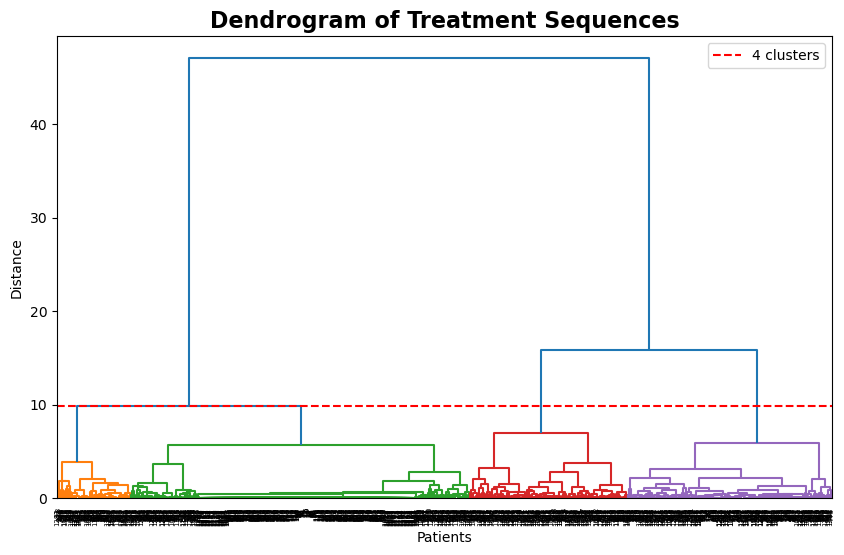
\includegraphics[width=\columnwidth]{dendrogramme_OM}
  \caption{Dendrogram of treatment sequences obtained by hierarchical agglomerative clustering (Ward's linkage) on the Optimal Matching distance matrix (1 317 patients, 18 months).}
  \label{fig:dendrogram}
\end{figure}

\begin{figure}[htbp]
  \centering
  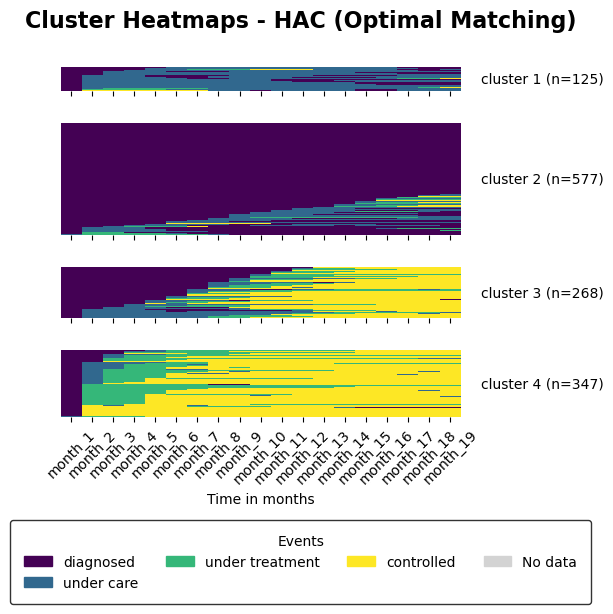
\includegraphics[width=\columnwidth]{cah_OM}
  \caption{Heatmaps of individual trajectories by cluster, obtained by hierarchical agglomerative clustering ($k = 4$) on the Optimal Matching distance matrix.}
  \label{fig:heatmap_cah}
\end{figure}

\FloatBarrier

\subsection{Multidimensional results}\label{sec:multi_res}

The multidimensional analysis was first conducted on a synthetic dataset generated via Synthea \citep{walonoski2020synthea}, comprising 901 patients with chronic conditions followed over 179 days.
The event types correspond to ten medications covering cardiovascular, respiratory, and metabolic treatments, including Albuterol and Fluticasone inhalers, Insulin, Metformin, Hydrochlorothiazide, Amlodipine, Atenolol, Nitroglycerin, and Simvastatin.
This controlled setting, with daily time granularity, a large number of event types, and a long observation period, provides a suitable starting point for exploring the behavior of \pkg{TCA} and validating the hyperparameter tuning workflow before applying it to real-world data.

The analysis was then extended to a real-world dataset consisting of oncological care trajectories from the VICAN5 survey (VIe 5 ans après le CANcer, a French national cohort of cancer survivors \cite{Bouhnike005971}), comprising 1 336 patients with colorectal cancer followed over 24 months.
In contrast to the Synthea dataset, trajectories are observed at monthly granularity over a shorter follow-up period, with only four event types corresponding to treatment modalities: intravenous chemotherapy, oral chemotherapy, surgery, and radiotherapy.
The larger patient cohort, combined with the sparsity and heterogeneity inherent to real clinical data, allows assessment of whether the conclusions drawn from the synthetic setting generalize to a more complex and realistic context.

In both cases, the goal is to extract a set of $R$ temporal phenotypes that jointly achieve high reconstruction quality and high phenotypic diversity.
Specifically, a good decomposition should satisfy two conditions: a $\text{FIT}_X$ value close to $1$, indicating that the phenotypes accurately reconstruct the observed trajectories, and a $\text{div}(\mathcal{P})$ value close to $1$, indicating that the extracted phenotypes capture distinct and complementary patterns of co-occurring clinical events.

In practice, these two objectives are often in tension: configurations that maximize $\text{FIT}_X$ tend to produce redundant phenotypes, while those that maximize diversity may sacrifice reconstruction quality.
The hyperparameter tuning process therefore aims to identify configurations that achieve a satisfactory balance between these two criteria, guiding the selection of $R$, $\omega$, $\tilde{\alpha}$, and $\tilde{\gamma}$.

\subsubsection{Synthea synthetic cohort}\label{sec:synthea_res}

\textbf{Experimental setup.}
The tensor constructed from the Synthea dataset has dimensions $K = 901$ patients, $n = 10$ event types, and a maximum duration of $T = 179$ days.
Each SWoTTeD trial runs for up to 500 epochs with early stopping (patience of 5 evaluations, monitored on $\text{FIT}_X$), a learning rate of $10^{-2}$, and a \emph{ReduceLROnPlateau} scheduler (factor 0.5, patience 10).

\textbf{Hyperparameter search.}
Ten configurations were sampled with \texttt{random.seed(42)} from the following space: rank $R \in \{2, \ldots, 5\}$, window length $\omega \in \{2, \ldots, 10\}$ days, normalised sparsity weight $\tilde{\alpha} \in [10^{-5},\, 2 \times 10^{-4}]$,
and normalised non-succession weight $\tilde{\gamma} \in [0.1,\, 2.0]$, both sampled on a log scale.
The rank upper bound was chosen to avoid empty or redundant phenotypes observed for higher ranks given the sparsity of the dataset.
The window length range was reduced after observing that only the first few days of longer windows were consistently activated.
The total search required approximately 1 360 minutes of computation.

The random search configurations were ranked by descending $\text{FIT}_X$, followed by descending $\text{div}(\mathcal{P})$ (Table~\ref{tab:results_synthea}). 
However, these metrics were used as quantitative criteria for ranking rather than as the sole basis for selecting the final configuration. 
The resulting phenotypes were also visually inspected to assess their interpretability and whether they represented distinct and meaningful patterns. 
Indeed, a configuration may achieve a high $\text{FIT}_X$ and high $\text{div}(\mathcal{P})$ while containing one or more phenotypes with little or no activation. 
In such cases, the diversity measure may remain high because it captures differences between the non-empty phenotypes and the inactive phenotype, despite the resulting decomposition providing limited interpretable information. 
Therefore, the final configuration was selected by jointly considering the quantitative metrics and the interpretability of the extracted phenotypes.
\begin{table}[htbp]
\centering
\caption{Random search results on the Synthea cohort, sorted by descending $\text{FIT}_X$ then descending $\text{div}(\mathcal{P})$.}
\label{tab:results_synthea}
\begin{tabular}{ccccccc}
\toprule
$R$ & $\omega$ & $\tilde{\alpha}$ & $\tilde{\gamma}$ & best $\text{FIT}_X$ & $\text{div}(\mathcal{P})$ & Time \\
\midrule
3 & 5 & $1.90$ & $0.91$ & $0.576$ & $0.972$ & $7 624$~s \\
2 & 2 & $3.74$ & $1.04$ & $0.572$ & $1.0$ & $7 873$~s \\
2 & 8 & $0.11$ & $0.66$ & $0.547$ & $0.999$ & $8 775$~s \\
5 & 3 & $0.57$ & $2.40$ & $0.535$ & $0.995$ & $9 000$~s \\
3 & 3 & $1.37$ & $4.83$ & $0.527$ & $0.957$ & $9 866$~s \\
5 & 5 & $0.25$ & $0.46$ & $0.461$ & $0.90$ & $8 842$~s \\
4 & 2 & $1.80$ & $1.25$ & $0.419$ & $0.854$ & $8 699$~s \\
2 & 8 & $0.14$ & $6.33$ & $0.414$ & $0.459$ & $8 993$~s \\
2 & 4 & $1.64$ & $1.39$ & $0.365$ & $0.879$ & $8 549$~s \\
3 & 10 & $0.33$ & $1.79$ & $0.038$ & $0.361$ & $3 413$~s \\
\bottomrule
\end{tabular}
\end{table}

\textbf{Results.}
The best configuration corresponds to $R = 3$, $\omega = 5$ days, $\tilde{\alpha} = 1.76 \times 10^{-4}$ and $\tilde{\gamma} = 2.74 \times 10^{-1}$, yielding absolute parameters $\alpha = 1.90$ and $\gamma = 9.14 \times 10^{-1}$,
$\text{FIT}_X = 0.576$ and $\text{div}(\mathcal{P}) = 0.972$.
Training ran for 150 epochs before early stopping was triggered (Figure~\ref{fig:training_synthea}).
$\text{FIT}_X$ increases steadily from 0.05 at epoch~10 to a peak of 0.576 around epoch~100, before declining as the non-succession regularisation term gains weight in the loss.
In the final epochs, the non-succession term $\gamma \cdot S(\mathcal{W})$ accounts for approximately 28\% of the total loss, while the sparsity term $\alpha \cdot \|\mathcal{P}\|_1$ remains marginal (around 3\%), indicating that the model is primarily constrained by the temporal succession penalty.

The three discovered phenotypes (Figure~\ref{fig:phenos_synthea}) capture distinct medication profiles.
\begin{itemize}
  \item \textbf{Phenotype~1} shows a faint signal on Atenolol Combo and Fluticasone Inhaler, suggesting a near-inactive or background profile.
  \item \textbf{Phenotype~2} is characterised by a strong and concentrated activation of Albuterol Inhaler and Fluticasone Inhaler over the $\omega = 5$-day window, corresponding to a respiratory treatment pattern.
  \item \textbf{Phenotype~3} captures a moderate activation of cardiovascular and metabolic medications (HCTZ~25mg, Insulin, Metformin), corresponding to a chronic disease management profile.
\end{itemize}

Reconstruction quality varies across patients depending on their medication profile.
For patient~18, whose trajectory is dominated by Albuterol Inhaler and Fluticasone Inhaler, the two medications captured by Phenotype~2, the reconstruction is very faithful, correctly recovering both the timing and the identity of medication episodes (Figure~\ref{fig:rec18_synthea}).
For patient~21, whose trajectory includes Atenolol Combo, Metformin, Insulin, and HCTZ~25mg, the reconstruction is less precise: the model captures the general temporal structure but attenuates or misplaces some events, reflecting the greater difficulty of reconstructing complex polypharmacy profiles with only three phenotypes (Figure~\ref{fig:rec21_synthea}).
This difference in reconstruction quality is consistent with the composition of the cohort: 586 out of 901 patients (65.0\%) received both Albuterol Inhaler and Fluticasone Inhaler during their follow-up, making the respiratory treatment pattern by far the most prevalent in the dataset and the dominant signal captured by Phenotype~2. 
Patients with more complex polypharmacy profiles, combining cardiovascular and metabolic medications such as Metformin, Insulin, or HCTZ, represent a smaller subgroup (at most 19.4\% of the cohort for Metformin), which
explains why Phenotype~3 captures these patterns with lower activation intensities and why their trajectories are reconstructed with less fidelity.

\textbf{Clustering.}
A pairwise Euclidean distance matrix was computed on the normalised phenotype intensity vectors, and hierarchical agglomerative clustering (HAC) with Ward linkage was applied.
The dendrogram (Figure~\ref{fig:dendro_synthea}) reveals a clear three-cluster structure.
The three clusters contain $n_1 = 508$, $n_2 = 304$, and $n_3 = 89$ patients respectively, as shown in the per-cluster heatmaps (Figure~\ref{fig:heatmap_synthea}).
\begin{itemize}
  \item Cluster~1 ($n_1 = 508$) is dominated by a strong activation of Phenotype~2, with Phenotypes~1 and~3 largely absent, corresponding to patients whose care pathway is primarily structured around respiratory medications (Albuterol and Fluticasone).
  \item Cluster~2 ($n_2 = 304$) presents moderate activations of both Phenotypes~2 and~3, with heterogeneous intensities, suggesting patients who combine respiratory and chronic disease medications.
  \item Cluster~3 ($n_3 = 89$) is characterised by a strong activation of Phenotype~1 and moderate activation of Phenotype~3, with Phenotype~2 essentially absent, corresponding to patients whose trajectory is dominated by cardiovascular and metabolic medications without significant respiratory treatment.
\end{itemize}

\begin{figure}[htbp]
    \centering
    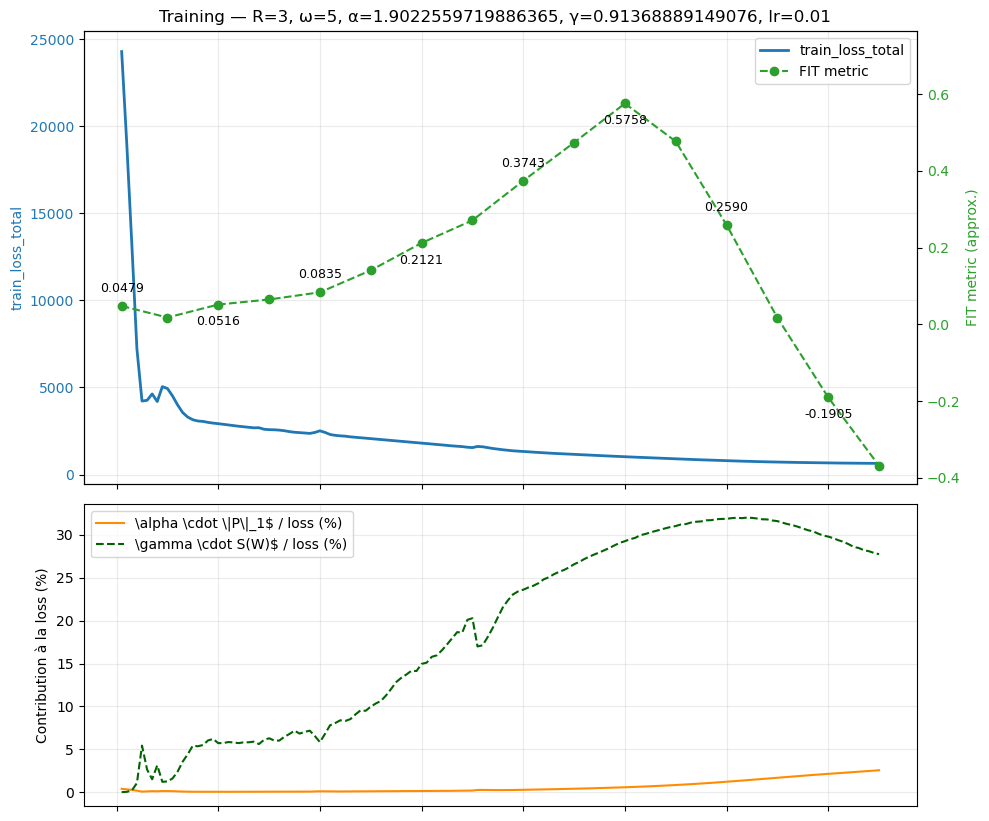
\includegraphics[width=\textwidth]{training_SYNTHEA.png}
    \caption{Training history of the retained SWoTTeD configuration on the Synthea cohort ($R=3$, $\omega=5$, $\alpha=1.90$, $\gamma=9.14\times10^{-1}$, $\text{lr}=10^{-2}$). 
    \textit{Top}: total training loss (blue) and approximate $\text{FIT}_X$ metric (green dashed) over 150 epochs.
    \textit{Bottom}: relative contributions of the sparsity term $\alpha\cdot\|\mathcal{P}\|_1$ (orange) and the non-succession term $\gamma\cdot S(\mathcal{W})$ (green dashed) to the total loss.}
    \label{fig:training_synthea}
\end{figure}

\begin{figure}[htbp]
    \centering
    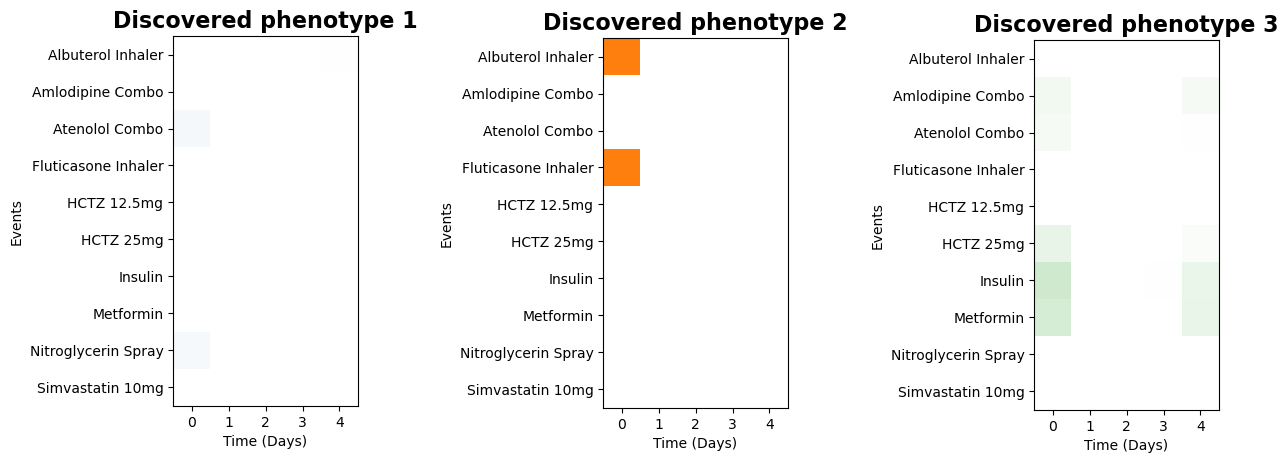
\includegraphics[width=\textwidth]{phenos_SYNTHEA.png}
    \caption{The three phenotypes discovered by SWoTTeD on the Synthea cohort ($R=3$, $\omega=5$, $\alpha=1.90$, $\gamma=9.14\times10^{-1}$, $\text{lr}=10^{-2}$).}
    \label{fig:phenos_synthea}
\end{figure}

\begin{figure}[htbp]
    \centering
    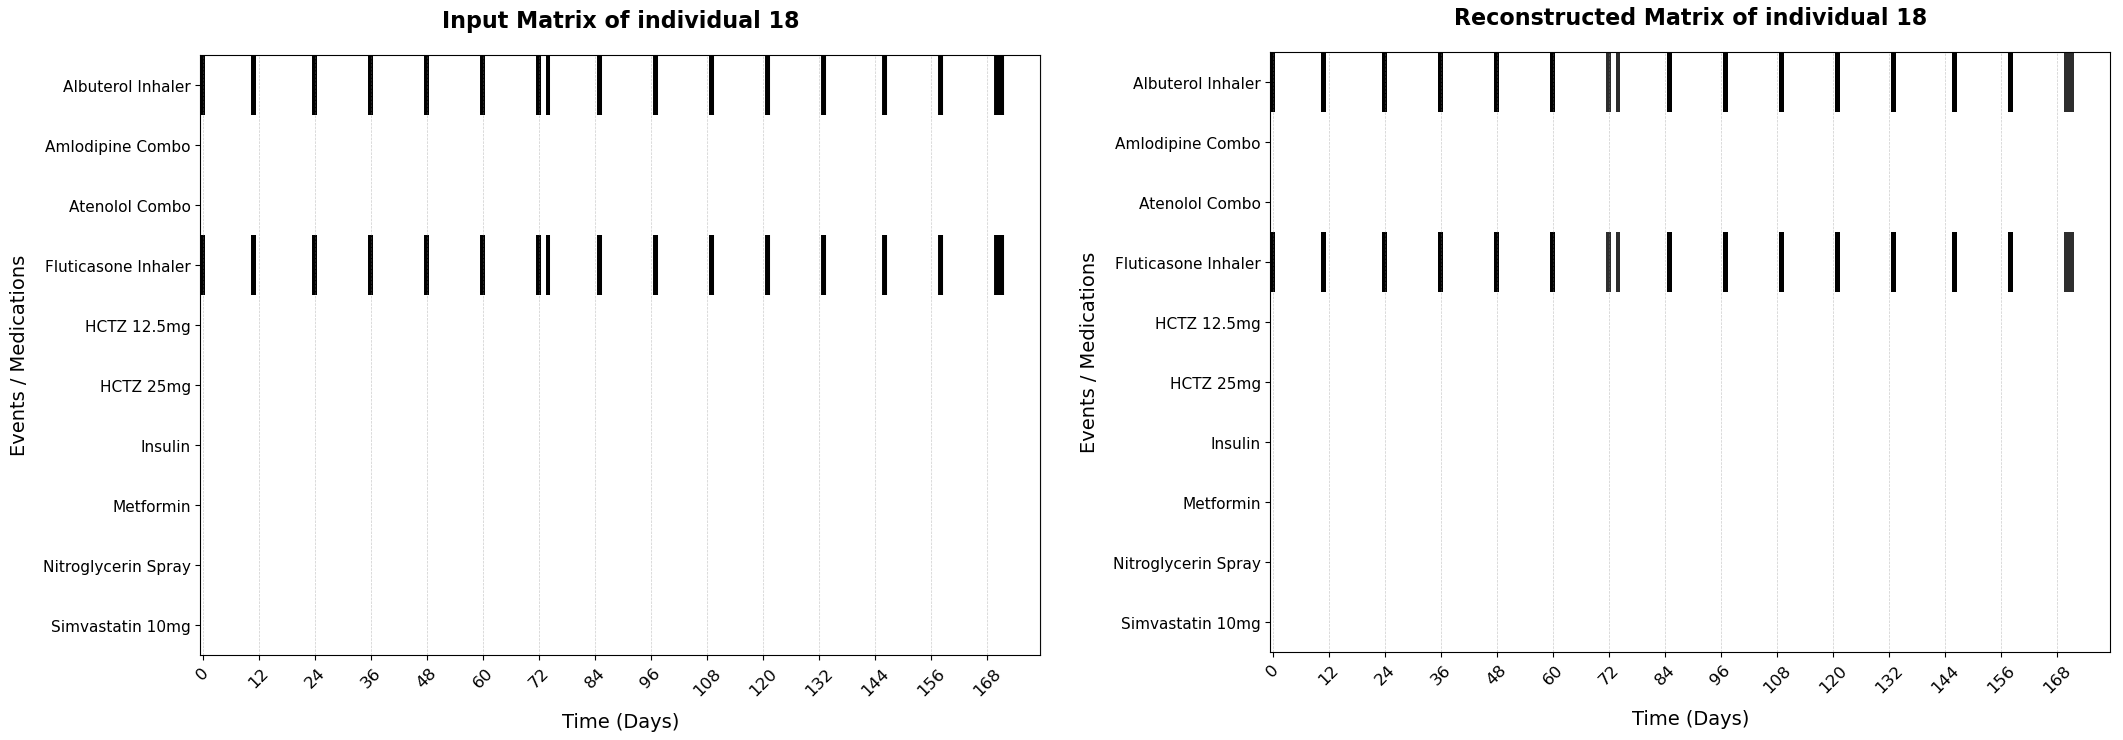
\includegraphics[width=\textwidth]{rec_pat18_SYNTHEA.png}
    \caption{Input matrix (left) and reconstructed matrix (right) for patient~18 in the Synthea cohort.}
    \label{fig:rec18_synthea}
\end{figure}

\begin{figure}[htbp]
    \centering
    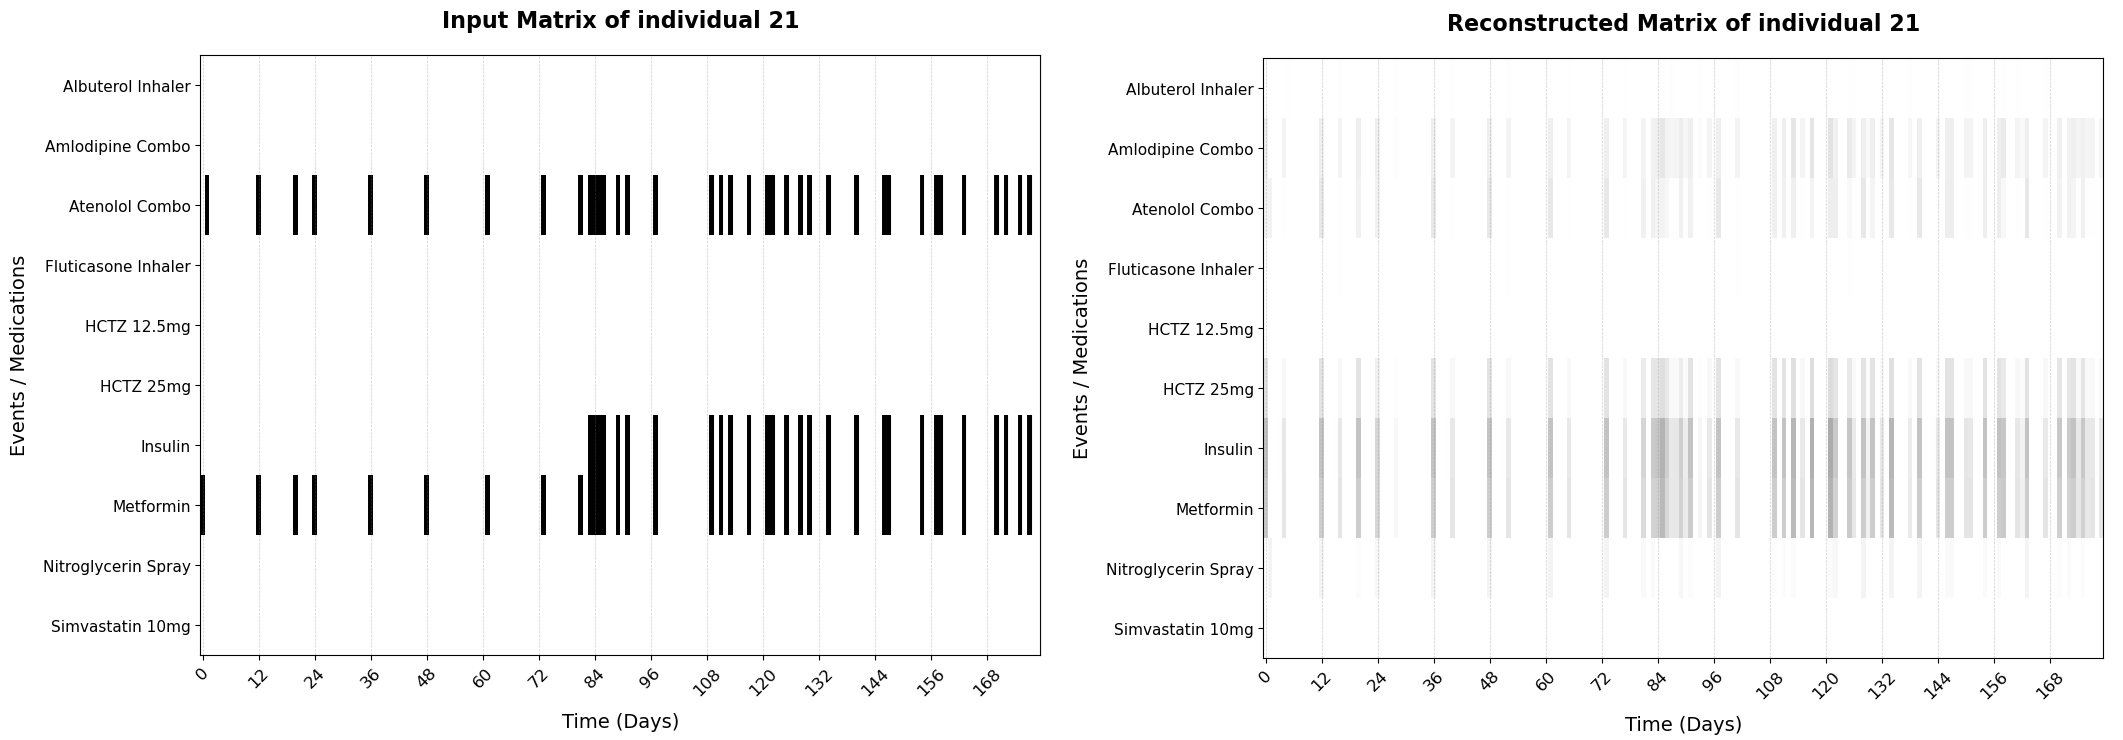
\includegraphics[width=\textwidth]{rec_pat21_SYNTHEA.png}
    \caption{Input matrix (left) and reconstructed matrix (right) for patient~21 in the Synthea cohort.}
    \label{fig:rec21_synthea}
\end{figure}

\begin{figure}[htbp]
    \centering
    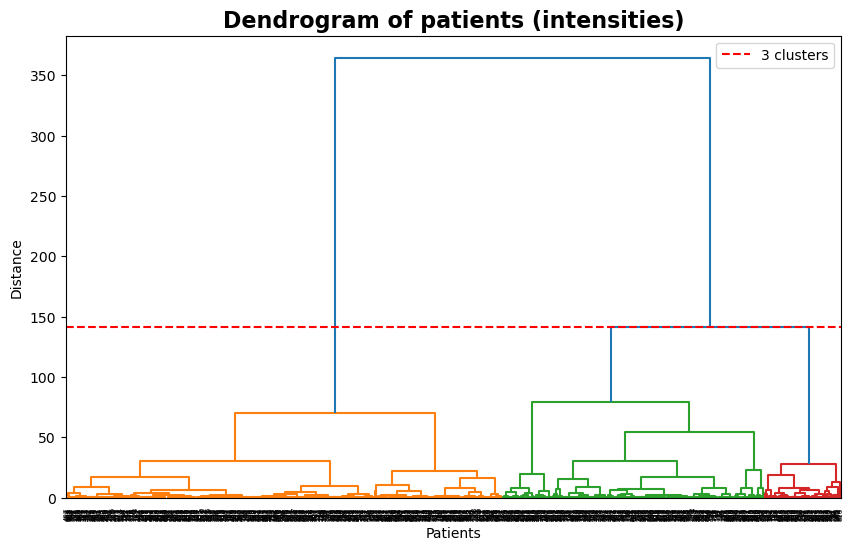
\includegraphics[width=\textwidth]{dendrogramme_SYNTHEA.png}
    \caption{Dendrogram of the 901 Synthea patients obtained by hierarchical agglomerative clustering (Ward linkage, Euclidean distance) applied to the normalised phenotype intensity vectors.}
    \label{fig:dendro_synthea}
\end{figure}

\begin{figure}[htbp]
    \centering
    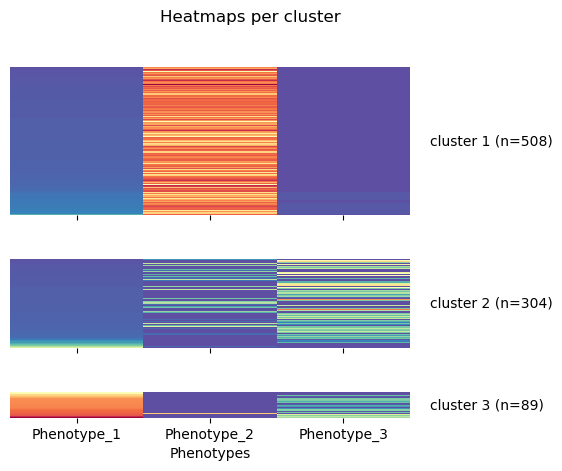
\includegraphics[width=0.85\textwidth]{heatmap_SYNTHEA.png}
    \caption{Per-cluster heatmaps of normalised phenotype intensities for the three patient clusters identified in the Synthea cohort. 
    Each row represents a patient, each column a phenotype, and the colour encodes the intensity of phenotype activation, ranging from low (dark blue) to high (dark red).}
    \label{fig:heatmap_synthea}
\end{figure}

\FloatBarrier

\subsubsection{VICAN5 real cohort}\label{sec:vican_res}

\textbf{Experimental setup.}
The tensor constructed from the VICAN5 dataset has dimensions $K = 1 336$ patients, $n = 4$ event, and a maximum follow-up duration of $\bar{T} = 24$ months.
Training settings are identical to those used for the Synthea cohort: up to 500 epochs, early stopping with patience of 5 epochs monitored on $\text{FIT}_X$, a learning rate of $10^{-2}$, and a \emph{ReduceLROnPlateau} scheduler.

\textbf{Hyperparameter search.}
A random search over 10 configurations was performed with \texttt{random.seed(42)}, drawing configurations uniformly from the following space: rank $R \in \{2, \ldots, 5\}$, window length $\omega \in \{2, \ldots, 5\}$ months, 
normalised sparsity weight $\tilde{\alpha} \in [10^{-5},\, 10^{-3}]$, and normalised non-succession weight $\tilde{\gamma} \in [0.1,\, 10.0]$, both sampled on a log scale.
The rank was bounded above by the number of treatment modalities ($n = 4$) to avoid phenotypes that cannot be meaningfully distinguished.
The window length upper bound reflects the typical duration of a treatment episode in colorectal cancer care.
The total search required approximately 29 hours of computation.

\textbf{Results.}
The configuration retained for interpretation ranked sixth by $\text{FIT}_X$ but was selected on the basis of phenotypic interpretability.
It uses rank $R = 3$, window length $\omega = 3$ months, normalised weights $\tilde{\alpha} = 0.28$ and $\tilde{\gamma} = 0.36$, corresponding to absolute regularisation parameters $\alpha = 7.91 \times 10^{-5}$, $\gamma = 0.36$.

The training history (Figure~\ref{fig:training_vican5}) illustrates the joint evolution of the total loss, $\text{FIT}_X$, and the two regularisation terms over 110 epochs.
The total loss decreases steadily from approximately 9000 at epoch~1 to around 1000 at convergence.
$\text{FIT}_X$ increases from 0.02 to a peak of 0.52 around epoch~60, before declining as the non-succession regularisation term $\gamma \cdot S(\mathcal{W})$ begins to dominate the loss budget, eventually stabilising at $\text{FIT}_X = 0.441$.
The retained configuration achieves a phenotypic diversity $\text{div}(\mathcal{P}) = 1.0$, confirming that the three discovered phenotypes are well separated in phenotype space.

The three discovered phenotypes (Figure~\ref{fig:phenos_vican5}) are clinically interpretable.
\begin{itemize}
  \item \textbf{Phenotype~1} captures moderate simultaneous oral chemotherapy and radiotherapy activation concentrated at month~0; 
  \item \textbf{Phenotype~2} shows strong, sustained intravenous chemotherapy activation over the full $\omega = 2$-month window.
  \item \textbf{Phenotype~3} corresponds to moderate surgical activation at month~0; 
\end{itemize}

The reconstruction of individual trajectories is overall satisfactory. 
For patient~8 (Figure~\ref{fig:rec_vican5}), the reconstructed matrix faithfully recovers the dominant temporal structure of the original trajectory, correctly localising the IV chemotherapy period (months~3--10) and the early treatment events at month~0. 
The activations are somewhat attenuated relative to the binary input, but the overall temporal pattern is well preserved.

\textbf{Clustering.}
A pairwise Euclidean distance matrix was computed on the normalised phenotype intensity vectors, and hierarchical agglomerative clustering (HAC) with Ward linkage was applied.
The dendrogram (Figure~\ref{fig:dendro_vican5}) reveals a clear four-cluster structure.

The four clusters contain patients with differents types of trajectories, as shown in the per-cluster heatmaps (Figure~\ref{fig:heatmap_vican5}).
\begin{itemize}
  \item Cluster~1 ($n_1 = 212$) shows very strong Phenotype~2 (IV chemotherapy) showing a cluster of patients only receiving IV chemotherapy, with very weak activations of Phenotypes~1 and~3 (oral chemotherapy, radiotherapy, and surgery); 
  \item Cluster~2 ($n_2 = 551$) shows a moderate activation of Phenotype~2 (IV chemotherapy) with weak activations of Phenotype~3 (surgery) and even weaker activation of Phenotype~1 (oral chemotherapy and radiotherapy); 
  \item Cluster~3 ($n_3 = 371$) shows Phenotype~3 (surgery), containing the patients that only had to have surgery in their treatments;
  \item Cluster~4 ($n_4 = 202$) shows low activation of Phenotype~1 (oral chemotherapy and radiotherapy).
\end{itemize}

\begin{figure}[htbp]
    \centering
    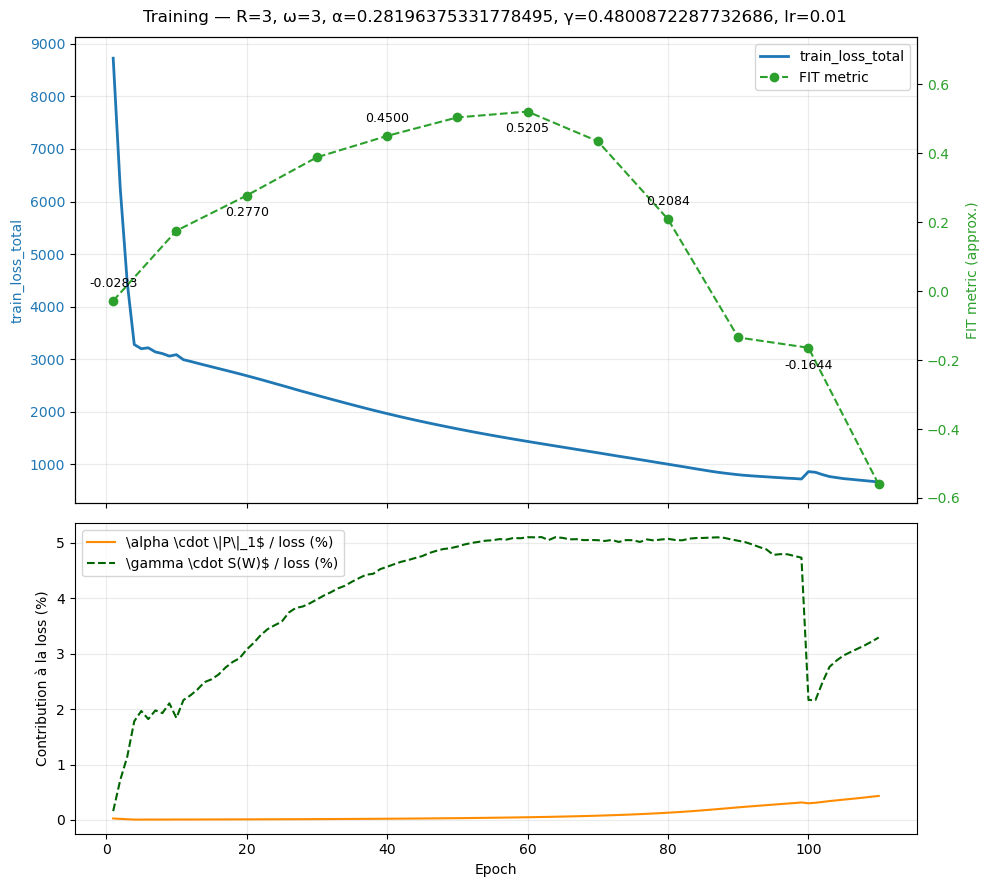
\includegraphics[width=\textwidth]{training_VICAN.png}
    \caption{Training history of the retained SWoTTeD configuration on the VICAN5 cohort ($R=3$, $\omega=3$, $\tilde{\alpha}=0.282$, $\tilde{\gamma}=0.480$, $\text{lr}=10^{-2}$). 
    \textit{Top}: total training loss (blue) and approximate $\text{FIT}_X$ metric (green dashed) over 110 epochs. 
    \textit{Bottom}: relative contributions of the sparsity term $\alpha\cdot\|\mathcal{P}\|_1$ (orange) and the non-succession term $\gamma\cdot S(\mathcal{W})$ (green dashed) to the total loss.}
    \label{fig:training_vican5}
\end{figure}

\begin{figure}[htbp]
    \centering
    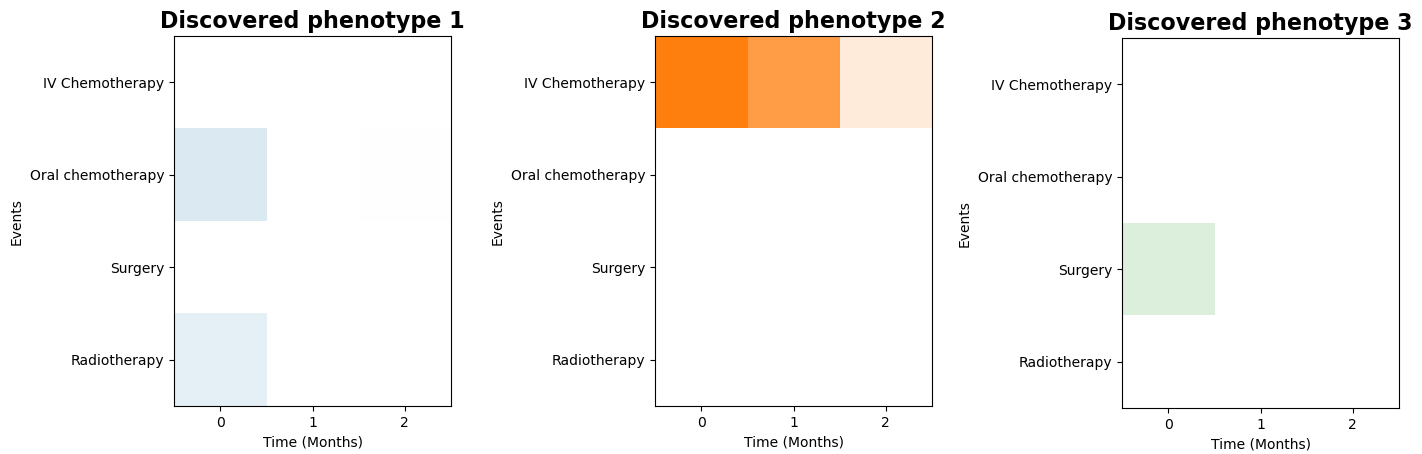
\includegraphics[width=\textwidth]{phenos_VICAN.png}
    \caption{The three phenotypes discovered by SWoTTeD on the VICAN5 cohort ($R=3$, $\omega=3$, $\tilde{\alpha}=0.282$, $\tilde{\gamma}=0.480$, $\text{lr}=10^{-2}$).}
    \label{fig:phenos_vican5}
\end{figure}

\begin{figure}[htbp]
    \centering
    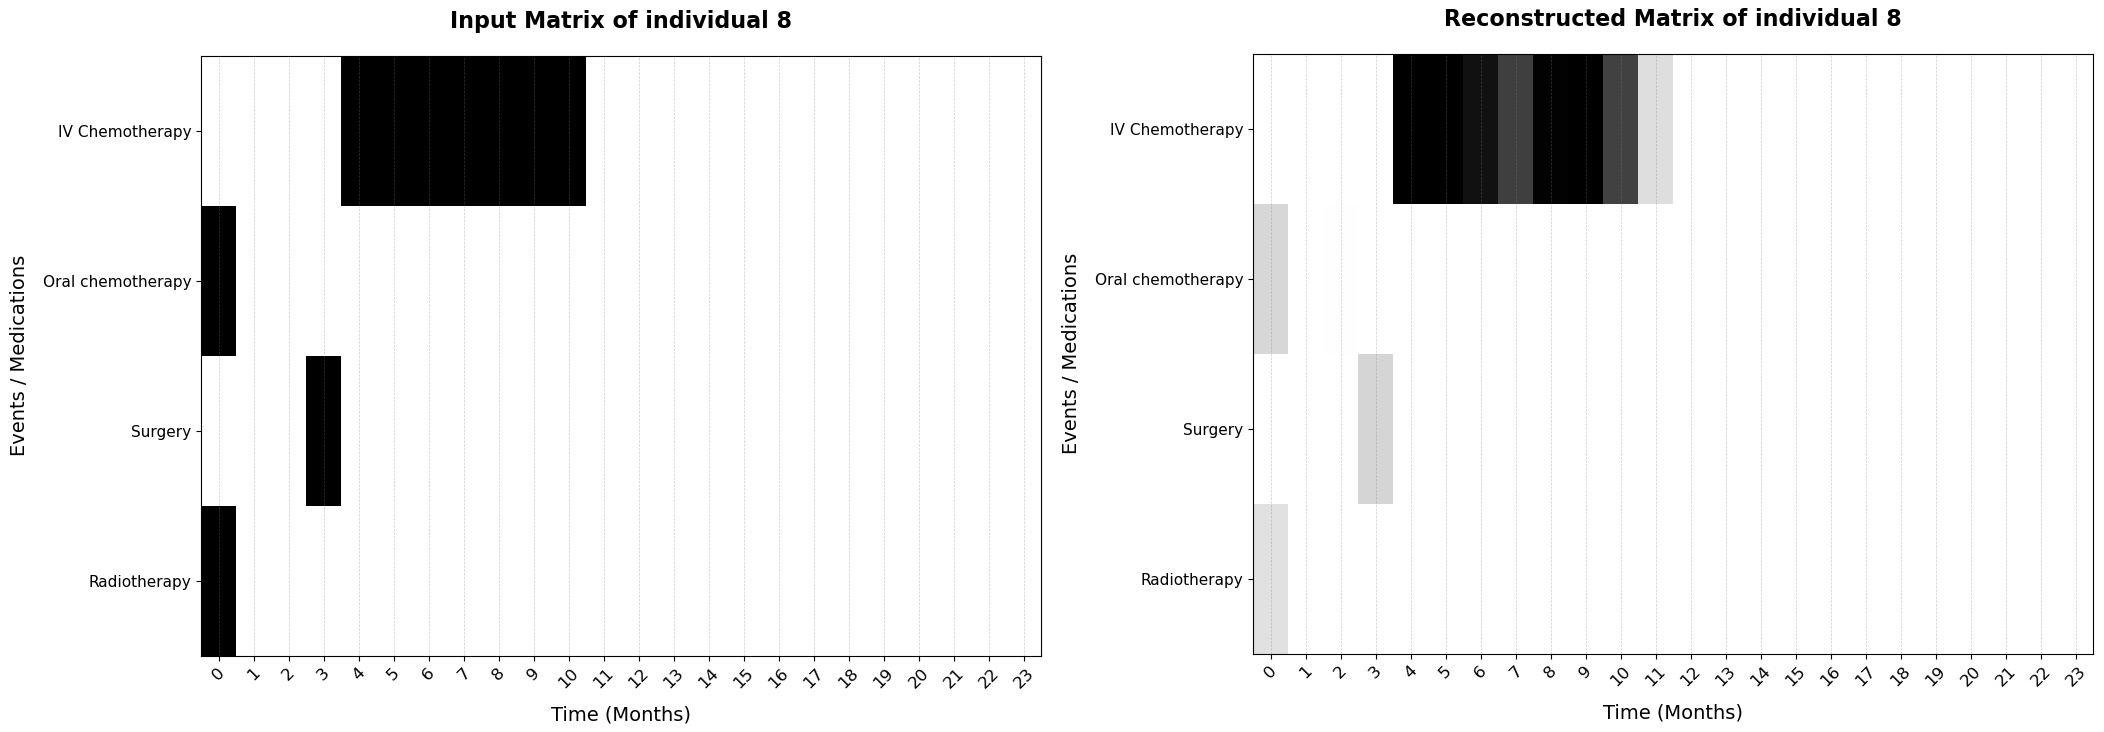
\includegraphics[width=\textwidth]{rec_pat8_VICAN.png}
    \caption{Input matrix (left) and reconstructed matrix (right) for patient~8 in the VICAN5 cohort.}
    \label{fig:rec_vican5}
\end{figure}

\begin{figure}[htbp]
    \centering
    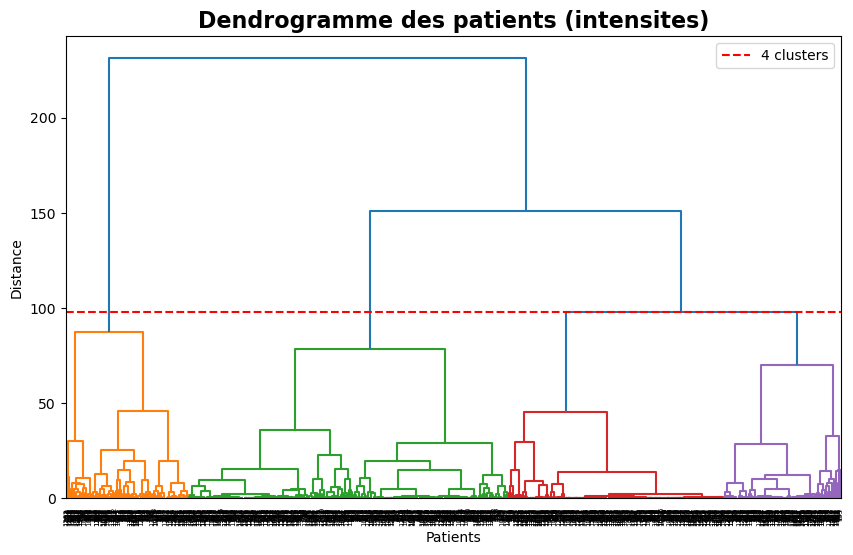
\includegraphics[width=\textwidth]{dendrogramme_VICAN.png}
    \caption{Dendrogram of the 1,336 VICAN5 patients obtained by hierarchical agglomerative clustering (Ward linkage, Euclidean distance) applied to the normalised phenotype intensity vectors. 
    The red dashed line indicates the cut of the at three clusters.}
    \label{fig:dendro_vican5}
\end{figure}

\begin{figure}[htbp]
    \centering
    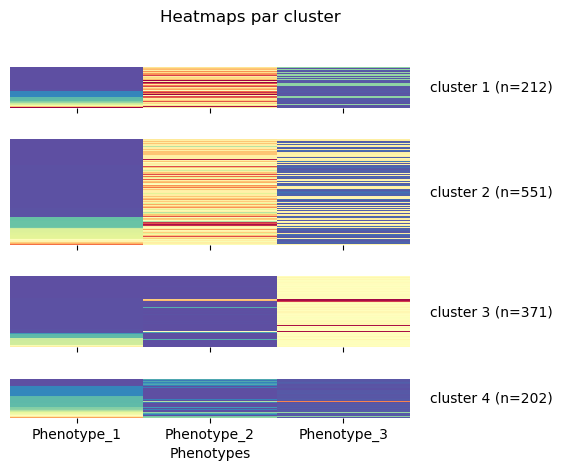
\includegraphics[width=0.85\textwidth]{heatmap_VICAN.png}
    \caption{Per-cluster heatmaps of normalised phenotype intensities for the three patient clusters identified in the VICAN5 cohort ($n_1=212$, $n_2=551$, $n_3=371$, $n_4=202$).
    Each row represents a patient, each column a phenotype, and the colour encodes the intensity of phenotype activation, ranging from low (dark blue) to high (dark red).}
    \label{fig:heatmap_vican5}
\end{figure}

\FloatBarrier

\section{Discussion}\label{sec:discussion}

\subsection{Unidimensional analysis}\label{sec:disc_uni}

\pkg{TCA} reproduced the four-cluster structure obtained with \pkg{TraMineR} on the same dataset, with clinically interpretable cluster profiles.
The \textit{Fast}, \textit{Slow}, \textit{Incomplete}, and \textit{Out of care} profiles correspond to distinct patterns of progression through the care continuum, including persistent disengagement from care and rapid progression toward controlled infection.

A limitation of the unidimensional module concerns the computation time of pairwise distance matrices: while most computations remain fast, DTW distance computation requires approximately 4~minutes and GAK distance computation approximately 6~minutes on the same dataset.. 
These costs are attributable to the quadratic complexity of pairwise distance computation and may take longer for larger cohorts.

\pkg{TraMineR}, a widely used tool for sequence analysis, is implemented in \proglang{R} and primarily supports unidimensional sequence representations. 
From a software perspective, \pkg{TCA} is, to our knowledge, the first \proglang{Python} package to offer a unified framework covering both unidimensional and multidimensional care trajectory analysis. 

\subsection{Multidimensional analysis}\label{sec:disc_multi}

\textbf{Computational cost.}
The SWoTTeD decomposition is computationally demanding, as each training run involves iterative gradient-based optimisation over a high-dimensional tensor.
Table~\ref{tab:compute_vican5} reports the computation times and parameters for the shortest and longest training runs observed on the VICAN5 cohort across the 10 random search configurations.
POURQUOI

\begin{table}[htbp]
\centering
\caption{Computation times and model characteristics for the shortest and longest training runs on the VICAN5 cohort ($K=1 336$ patients, $n=4$ event types, $\bar{T}=24$ months).}
\label{tab:compute_vican5}
\begin{tabular}{lcccccc}
\toprule
 & $R$ & $\omega$ & $\tilde{\alpha}$ & $\tilde{\gamma}$ & Time \\
\midrule
Shortest & $4$ & $3$ & $0.723$ & $2.527$ & $3 195$~s \\
Longest  & $2$ & $5$ & $0.050$ & $9.909$ & $7 555$~s \\
\bottomrule
\end{tabular}
\end{table}

\textbf{Balancing reconstruction quality, diversity, and interpretability.}
A central challenge in applying SWoTTeD to real-world data is finding a configuration that simultaneously achieves satisfactory reconstruction quality, diverse phenotypes, and clinically interpretable profiles.
These three objectives are not always aligned: configurations yielding high $\text{FIT}_X$ values may produce phenotypes that are too similar to be clinically distinguished, while configurations with high phenotypic diversity may do so at the cost of a poor reconstruction of the original trajectories.
Conversely, phenotypes that are visually sharp and interpretable do not always correspond to the configurations with the best numerical scores, as illustrated by the VICAN5 analysis where the retained configuration ranked sixth by $\text{FIT}_X$ yet produced the most clinically coherent phenotypic profiles.

On the Synthea cohort, $\text{FIT}_X$ values up to $0.576$ were achieved, consistent with the controlled nature of the synthetic data.
On the VICAN5 cohort, retained configurations reached $\text{FIT}_X$ values up to $0.58$, which is lower than the values around $0.7$ reported by \cite{sebia2024swotted} on other datasets.
The difference may reflect the greater heterogeneity and sparsity of real-world clinical trajectories, which makes reconstruction more challenging.

To navigate this trade-off in practice, several complementary strategies were implemented in \pkg{TCA}.
Early stopping monitored on $\text{FIT}_X$ limits continued optimisation when reconstruction quality no longer improves, preventing excessive optimisation of the regularisation terms at the expense of reconstruction quality.
A \emph{ReduceLROnPlateau} scheduler adaptively reduces the learning rate when progress in the monitored metric plateaus, which can help stabilise optimisation.
A phenotypic diversity metric $\text{div}(\mathcal{P})$ was added to the package to provide a quantitative measure of phenotype separation that can be tracked alongside $\text{FIT}_X$ during the random search.
However, these quantitative criteria are necessary but not sufficient: visual inspection of the discovered phenotypes remains essential, as configurations with similar numerical scores can yield phenotypes with very different clinical interpretability.
This observation supports the use of quantitative metrics as complementary criteria rather than as the sole basis for model selection.
This observation also points to a broader methodological consideration: automated hyperparameter optimisation in unsupervised trajectory analysis cannot fully replace domain knowledge. 
Integrating clinical expertise into model selection therefore remains an important step for obtaining meaningful and interpretable trajectory phenotypes.

\section{Conclusion}\label{sec:conclusion}

This study presented \pkg{TCA} (Trajectory Clustering Analysis), an open-source \proglang{Python} package providing a unified framework for the analysis of longitudinal care trajectories in both unidimensional and multidimensional settings.

The unidimensional module integrates multiple dissimilarity measures and clustering algorithms and was shown to recover clinically interpretable trajectory profiles on a real-world clinical sequence dataset.

The multidimensional module integrates the SWoTTeD tensor decomposition~\cite{sebia2024swotted}, extending the analysis to settings in which multiple care events may co-occur over time. 
Applied to both a synthetic cohort and a real-world colorectal cancer cohort, it identified distinct temporal phenotypes and supported the construction of clinically interpretable patient typologies.

These experiments also highlighted an important practical challenge in multidimensional trajectory analysis: reconstruction quality, phenotypic diversity, and clinical interpretability are not necessarily aligned. 
Consequently, hyperparameter selection cannot be based solely on a single numerical criterion, and visual inspection of the resulting phenotypes remains an important component of model selection.

Future methodological developments will focus on identifying more straightforward and data-adaptive strategies for hyperparameter selection, with the aim of reducing the computational cost and subjectivity of the model selection process.

More broadly, \pkg{TCA} is not restricted to oncology and can be applied to longitudinal biomedical datasets in which clinical or healthcare events are recorded over time. 
By bringing unidimensional trajectory clustering and multidimensional temporal tensor decomposition into a single \proglang{Python} framework, \pkg{TCA} aims to facilitate the application of advanced trajectory analysis methods in biomedical research.

\backmatter

\bmhead{List of abbreviations}
\begin{itemize}
  \item \textbf{TCA}: Trajectory Clustering Analysis
  \item \textbf{SWoTTeD}: Sliding Window for Temporal Tensor Decomposition
  \item \textbf{OM}: Optimal Matching
  \item \textbf{DTW}: Dynamic Time Warping
  \item \textbf{GAK}: Global Alignment Kernel
  \item \textbf{HAC}: Hierarchical Agglomerative Clustering
  \item \textbf{FIT}: Fit metric of the tensor decomposition (reconstruction quality metric)
  \item \textbf{LLM}: Large Language Model
  \item \textbf{VICAN5}: Vie après le CANcer, 5-year survey
  \item \textbf{CCTIRS}: Comité Consultatif sur le Traitement de l'Information en Matière de Recherche dans le Domaine de la Santé
  \item \textbf{CNIL}: Commission Nationale de l'Informatique et des Libertés
  \item \textbf{ISP}: Institute of Public Health
\end{itemize}

\bmhead{Availability and requirements}
\begin{itemize}
  \item \textbf{Project name:} TCA (Trajectory Clustering Analysis)
  \item \textbf{Project home page:} \url{https://github.com/QuanTIMLab/TrajectoryClusteringAnalysis}
  \item \textbf{Operating system:} Platform independent
  \item \textbf{Programming language:} Python $\geq$ 3.6
  \item \textbf{License:} MIT
\end{itemize}

\bmhead{Declarations}
\begin{itemize}
  \item \textbf{Ethics approval and consent to participate:} The Synthea \citep{walonoski2020synthea} dataset is fully synthetic and contains no real human data.
  The \textit{unidimensional\_data} dataset is an open-access educational dataset provided by Larmarange \citep{larmarange_analyseR} for statistical training purposes. It is distributed for methodological demonstration without identifiable personal data.
  The VICAN5 \citep{Bouhnike005971} dataset was collected as part of a national survey whose methodology was approved by three national ethics commissions: 
  the CCTIRS (Comité Consultatif sur le Traitement de l’Information en Matière de Recherche dans le Domaine de la Santé, study registered under no. 11-143), 
  the ISP (Institute of Public Health, study registered under no. C11-63) 
  and the CNIL (French Commission on Individual Data Protection and Public Liberties, study registered under no. 911290). 
  Confidentiality is assured for all participants with regard to any personal responses and information provided, as all data collected are anonymised.
  \item \textbf{Consent for publication:} Not applicable
  \item \textbf{Availability of data and materials:} The datasets used and analysed during the current study are available at \url{https://github.com/QuanTIMLab/TrajectoryClusteringAnalysis}
  \item \textbf{Competing interests:} The authors declare that they have no competing interests
  \item \textbf{Funding:} A REMPLIR
  \item \textbf{Authors' contributions:} A REMPLIR
  \item \textbf{Acknowledgements:} A REMPLIR
\end{itemize}

\bibliography{bib}

\end{document}